\cleardoublepage
\chapter{PERANCANGAN SISTEM \textit{SMART WASTE BIN}}
\label{chap:perancangan}

Bab ini merupakan bagian dari fase perancangan dan pengembangan dalam metodologi \textit{Design Science Research} yang telah diuraikan pada Subbab I.5.2. Berdasarkan hasil analisis kebutuhan dan pemilihan solusi pada Bab III, dirancang sistem pemantauan sampah berbasis \textit{Internet of Things} yang terdiri dari perangkat IoT, \textit{middleware}, \textit{database}, dan \textit{dashboard}.

Komponen sistem dibedakan menjadi dua kategori: komponen eksternal berupa perangkat IoT \textit{Smart Waste Bin} dari pihak ketiga, serta komponen internal yang dikembangkan oleh peneliti meliputi \textit{middleware}, \textit{database}, dan \textit{dashboard}. Karena konfigurasi \textit{firmware} bawaan perangkat dirancang untuk skala perkotaan sebagaimana diidentifikasi pada Subbab \ref{sec:analisis-kondisi}, bab ini juga menjelaskan perancangan adaptasi \textit{firmware} yang dilakukan agar perangkat dapat beroperasi optimal di lingkungan kampus.

% ============================================================
\section{Gambaran Umum Sistem}
\label{sec:gambaran-umum}
% ============================================================

Subbab ini menyajikan gambaran umum sistem pemantauan sampah berbasis \textit{Internet of Things} yang dikembangkan, mencakup arsitektur sistem secara keseluruhan, alur data dari pengumpulan hingga analisis, dan pemilihan teknologi. Gambaran umum ini bertujuan untuk memberikan pemahaman holistik mengenai struktur dan cara kerja sistem secara konseptual sebelum membahas perancangan detail pada subbab-subbab selanjutnya.

\subsection{Arsitektur Sistem}

Sistem Pemantauan Sampah Berbasis \textit{Internet of Things} dirancang menggunakan arsitektur berlapis (\textit{layered architecture}) yang mengacu pada model arsitektur IoT. Berbeda dengan model \textit{three-layer architecture} standar, sistem ini mengadopsi \textit{four-layer architecture} dengan penambahan \textit{Middleware Layer}. Pemilihan arsitektur empat \textit{layer} didasarkan pada kebutuhan untuk memisahkan fungsi transmisi data dengan fungsi pemrosesan dan \textit{routing} data, sehingga memberikan modularitas yang lebih baik dalam pengembangan dan pemeliharaan sistem.

Gambar \ref{fig:arsitektur-sistem} menunjukkan arsitektur keseluruhan sistem pemantauan sampah berbasis \textit{Internet of Things} yang terdiri dari empat \textit{layer} utama beserta pembagian komponen berdasarkan tanggung jawab pengembangan.

\begin{figure}[H]
  \caption{Arsitektur Sistem Pemantauan Sampah Berbasis \textit{Internet of Things}}
  \label{fig:arsitektur-sistem}
  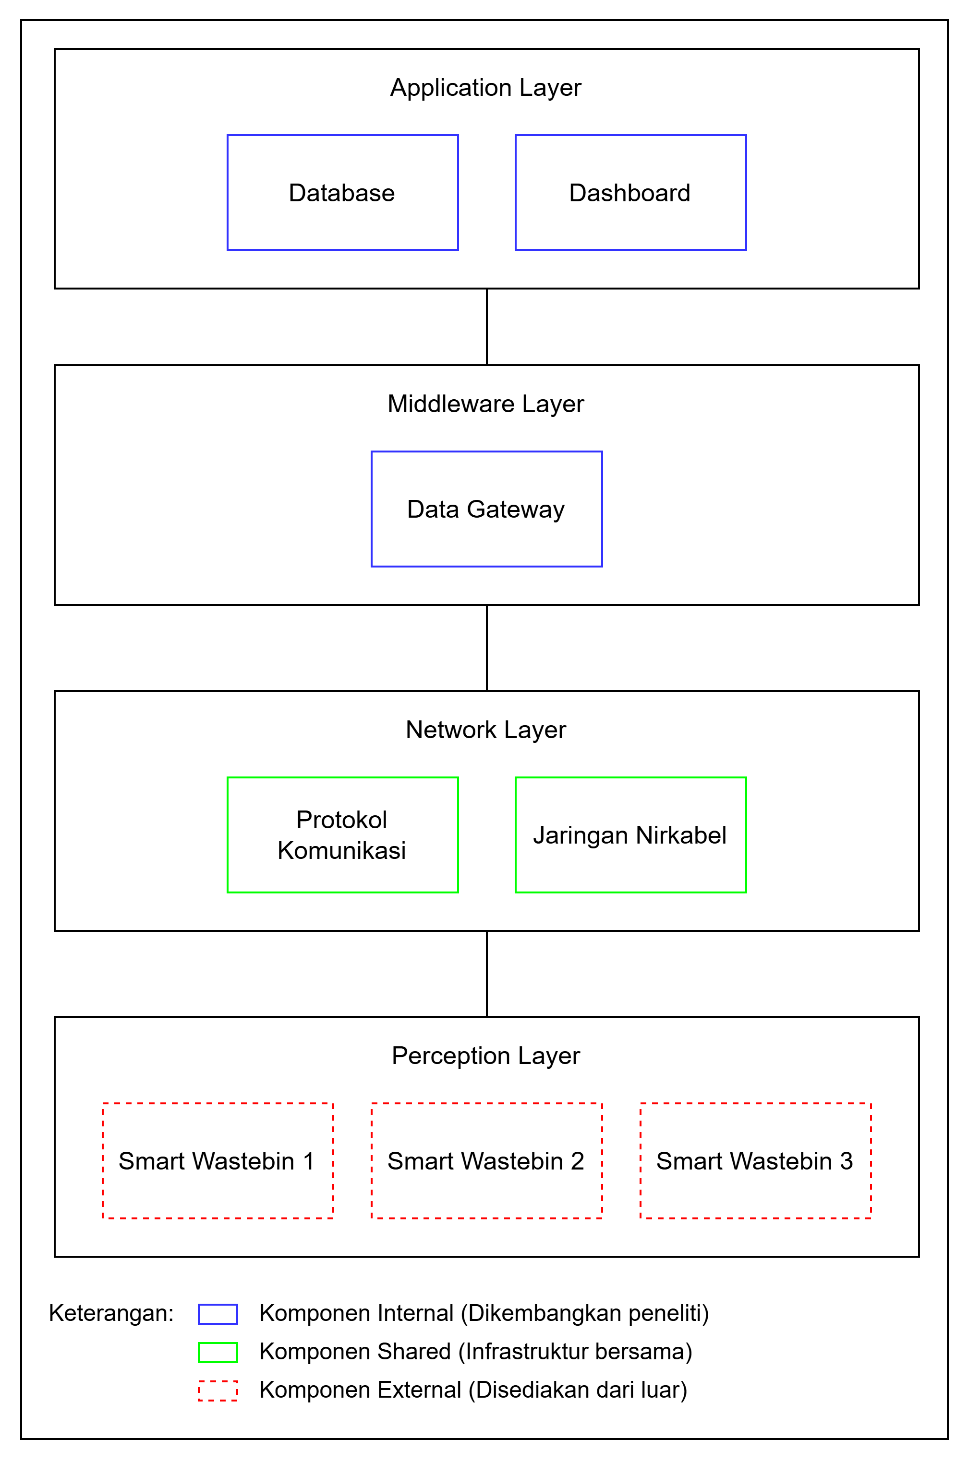
\includegraphics[width=0.7\textwidth]{images/arsitektur-sistem.png}
  % RENAME: image7.png → arsitektur-sistem.png
\end{figure}

Berdasarkan Gambar \ref{fig:arsitektur-sistem}, sistem terdiri dari empat \textit{layer} dengan fungsi sebagai berikut.

\begin{enumerate}
  \item \textit{Perception Layer}: terdiri dari tiga unit perangkat \textit{Smart Waste Bin} yang berfungsi mengumpulkan data tingkat kepenuhan tempat sampah secara periodik.
  \item \textit{Network Layer}: menyediakan infrastruktur komunikasi nirkabel untuk mentransmisikan data dari perangkat ke sistem penerima.
  \item \textit{Middleware Layer}: merupakan penambahan dari arsitektur standar, berfungsi sebagai data \textit{gateway} yang menerima, memvalidasi, dan meneruskan data ke \textit{layer} di atasnya.
  \item \textit{Application Layer}: terdiri dari dua komponen utama yaitu sistem \textit{database} untuk penyimpanan data dan \textit{dashboard} untuk visualisasi serta analisis pola pembuangan sampah.
\end{enumerate}

Arsitektur sistem juga membedakan komponen berdasarkan tanggung jawab pengembangan. Komponen eksternal mencakup perangkat IoT pada \textit{Perception Layer} yang disediakan oleh vendor. Komponen internal mencakup data \textit{gateway} pada \textit{Middleware Layer} serta seluruh komponen pada \textit{Application Layer} yang dikembangkan oleh peneliti. Komponen \textit{shared} mencakup infrastruktur \textit{Network Layer} yang digunakan bersama.

\subsection{Alur Data Sistem}

Sistem Pemantauan Sampah Berbasis \textit{Internet of Things} mengimplementasikan alur data yang terstruktur dari pengumpulan data di perangkat IoT hingga penyajian informasi kepada pengguna. Untuk menggambarkan alur data secara sistematis, digunakan \textit{Data Flow Diagram} (DFD) yang terdiri dari dua level: DFD Level 0 (\textit{Context Diagram}) dan DFD Level 1.

DFD Level 0 menggambarkan sistem pemantauan sampah berbasis \textit{Internet of Things} sebagai satu kesatuan proses yang berinteraksi dengan entitas eksternal, sebagaimana ditunjukkan pada Gambar \ref{fig:dfd-level0}.

\begin{figure}[H]
  \caption{\textit{Data Flow Diagram} Level 0}
  \label{fig:dfd-level0}
  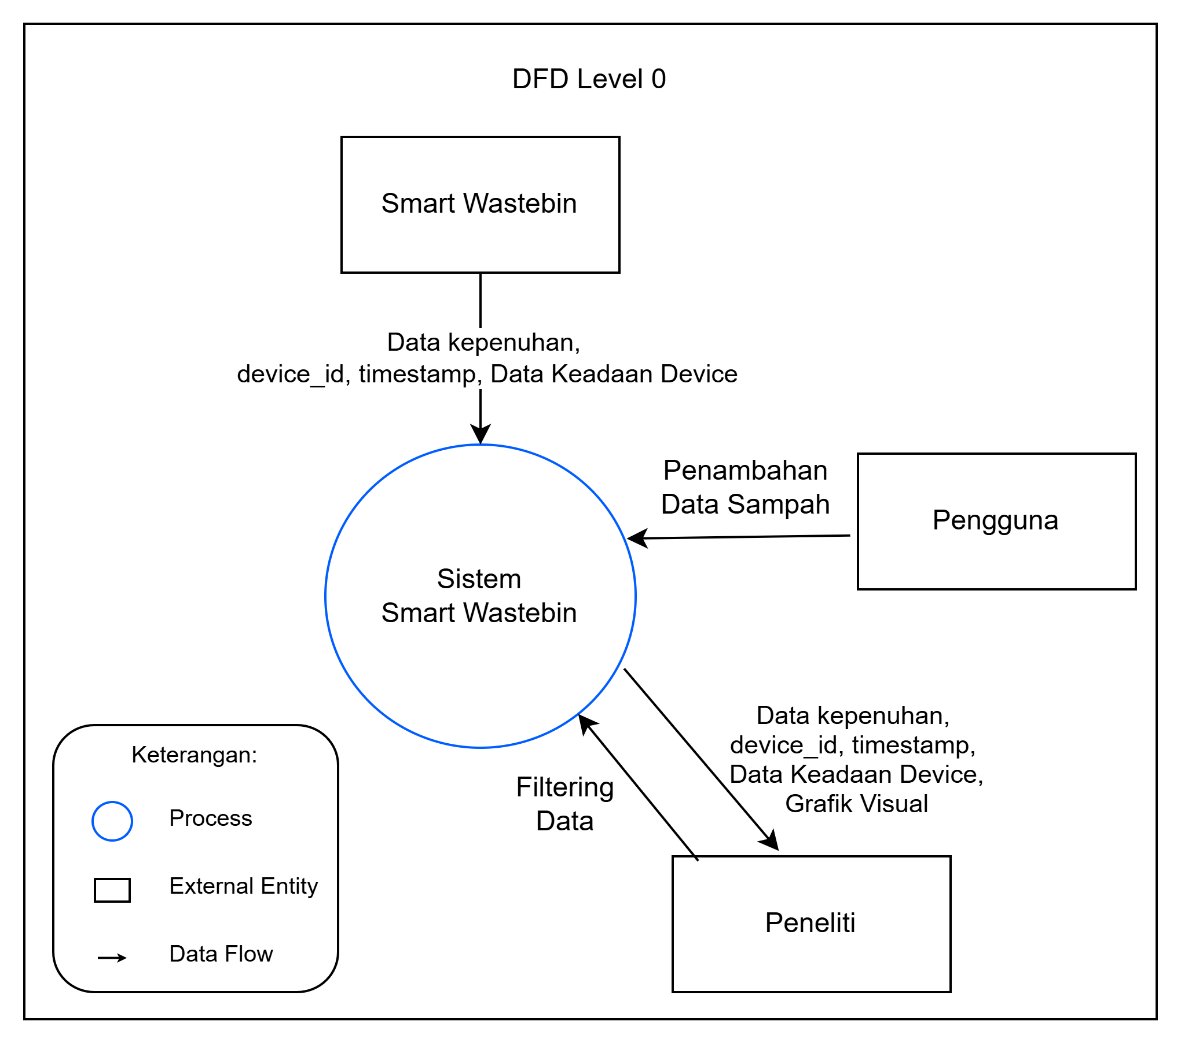
\includegraphics[width=0.85\textwidth]{images/dfd-level0.png}
  % RENAME: image8.png → dfd-level0.png
\end{figure}

Berdasarkan Gambar \ref{fig:dfd-level0}, terdapat dua entitas eksternal yang berinteraksi dengan sistem. Pertama, \textit{Smart Waste Bin} sebagai perangkat IoT sumber data yang mengirimkan data tingkat kepenuhan, identifier perangkat, dan \textit{timestamp} pembacaan secara periodik. Kedua, Pengguna yang mencakup pengelola gedung dan peneliti, yang mengirimkan \textit{request} data dan \textit{filter}, kemudian menerima visualisasi status dan grafik historis sebagai \textit{output}. Analisis pola terhadap data yang tersimpan dilakukan secara terpisah oleh peneliti, di luar alur operasional sistem.

DFD Level 1 menunjukkan dekomposisi proses tunggal pada DFD Level 0 menjadi tiga proses utama, sebagaimana ditunjukkan pada Gambar \ref{fig:dfd-level1}.

\begin{figure}[H]
  \caption{\textit{Data Flow Diagram} Level 1}
  \label{fig:dfd-level1}
  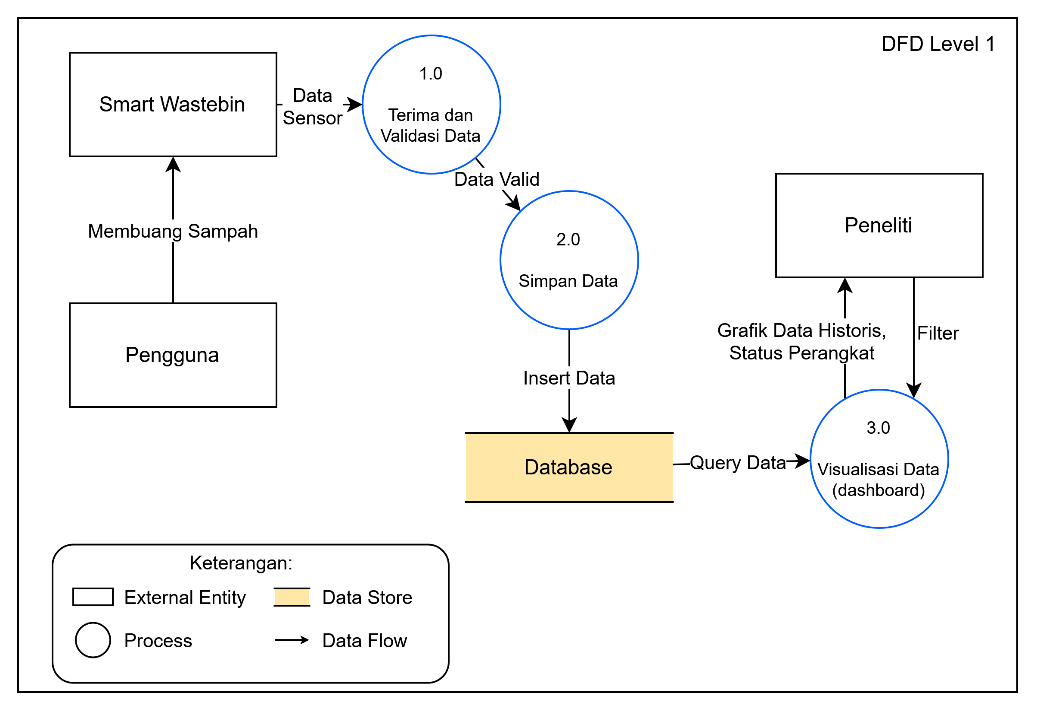
\includegraphics[width=0.85\textwidth]{images/dfd-level1.png}
  % RENAME: image9.png → dfd-level1.png
\end{figure}

Tabel \ref{tab:dfd-komponen} menyajikan deskripsi setiap komponen dalam DFD Level 1.

\begin{table}[H]
  \caption{Deskripsi Komponen DFD Level 1}
  \label{tab:dfd-komponen}
  \begin{tabularx}{\textwidth}{| l | l | l | X |}
    \hline
    \textbf{ID} & \textbf{Komponen} & \textbf{Tipe} & \textbf{Deskripsi} \\
    \hline
    1.0 & Terima \& Validasi Data & Proses & Menerima data dari perangkat IoT, melakukan \textit{parsing} dan validasi format serta nilai data \\
    \hline
    2.0 & Simpan Data & Proses & Menyimpan data yang telah tervalidasi ke dalam \textit{database} secara persisten melalui \textit{middleware} \\
    \hline
    3.0 & Visualisasi Data & Proses & Mengambil data dari \textit{database}, menyajikan dalam bentuk \textit{dashboard} dan grafik, serta memberikan status perangkat untuk kebutuhan pemeliharaan \\
    \hline
    D1 & \textit{Database} & Data Store & Menyimpan seluruh data pembacaan sensor secara historis \\
    \hline
  \end{tabularx}
\end{table}

Tabel \ref{tab:dfd-alur} menjelaskan setiap alur data yang dilalui dalam sistem.

\begin{table}[H]
  \caption{Alur Data DFD Level 1}
  \label{tab:dfd-alur}
  \begin{tabularx}{\textwidth}{| l | l | l | X |}
    \hline
    \textbf{No} & \textbf{Dari} & \textbf{Ke} & \textbf{Data yang Mengalir} \\
    \hline
    1 & \textit{Smart Waste Bin} & Proses 1.0 & Data sensor (\textit{fillLevel}, \textit{sensor\_id}, \textit{timestamp}, \textit{battery}, dll.) \\
    \hline
    2 & Proses 1.0 & Proses 2.0 & Data tervalidasi \\
    \hline
    3 & Proses 2.0 & \textit{Database} & Record data pembacaan \\
    \hline
    4 & \textit{Database} & Proses 3.0 & \textit{Query result} (data sesuai \textit{filter}) \\
    \hline
    5 & Proses 3.0 & Pengguna & \textit{Dashboard}, grafik historis, status perangkat \\
    \hline
    6 & Pengguna & Proses 3.0 & \textit{Request} data, parameter \textit{filter}, rentang waktu \\
    \hline
  \end{tabularx}
\end{table}

Selain DFD yang menggambarkan aliran data secara fungsional, alur data secara teknis end-to-end disajikan pada Gambar \ref{fig:data-workflow}. Diagram ini menunjukkan perjalanan data konkret mulai dari pembacaan sensor pada perangkat IoT, transmisi melalui MQTT, pemrosesan pada \textit{middleware} Node-RED, penyimpanan pada \textit{database} Supabase, hingga penyajian pada \textit{dashboard}, beserta format data dan mekanisme penanganan \textit{error} pada setiap tahap.

\begin{figure}[H]
  \caption{Alur Data (\textit{Data Workflow}) Sistem}
  \label{fig:data-workflow}
  \centering
  \includegraphics[width=0.92\textwidth]{images/data-workflow.png}
\end{figure}

Untuk memberikan gambaran menyeluruh mengenai cara kerja sistem dalam konteks penelitian, Gambar \ref{fig:sistem-workflow} menyajikan alur kerja keseluruhan (\textit{workflow}) yang dipetakan terhadap fase-fase metodologi \textit{Design Science Research}. Diagram ini menegaskan pembagian peran antara sistem dan peneliti: sistem berperan pada fase perancangan-pengembangan dan demonstrasi (membangun serta mengumpulkan dan menyajikan data), sedangkan peneliti berperan pada fase evaluasi dan komunikasi (menganalisis data dan menyimpulkan).

\begin{figure}[H]
  \caption{Alur Kerja Keseluruhan Sistem (\textit{Workflow})}
  \label{fig:sistem-workflow}
  \centering
  \includegraphics[width=0.95\textwidth]{images/sistem-workflow.png}
\end{figure}

\subsection{Pemilihan Teknologi}

Pemilihan teknologi didasarkan pada beberapa pertimbangan: kesesuaian dengan kebutuhan fungsional dan nonfungsional pada Bab III, kemudahan integrasi antar komponen, ketersediaan dokumentasi dan dukungan komunitas, serta pengalaman pengembang. Tabel \ref{tab:pemilihan-teknologi} menyajikan teknologi yang digunakan pada setiap \textit{layer} sistem beserta justifikasinya.

\begin{longtable}{| l | l | l | p{5cm} |}
  \caption{Pemilihan Teknologi}
  \label{tab:pemilihan-teknologi} \\
    \hline
    \textbf{\textit{Layer}} & \textbf{Komponen} & \textbf{Teknologi} & \textbf{Justifikasi} \\
    \hline
  \endfirsthead
    \hline
    \textbf{\textit{Layer}} & \textbf{Komponen} & \textbf{Teknologi} & \textbf{Justifikasi} \\
    \hline
  \endhead
    \hline
  \endfoot
    \textit{Perception} & Mikrokontroler & ESP32 & \textit{Dual-core processor}, konsumsi daya rendah dengan \textit{deep sleep mode} \\
    \hline
    \textit{Perception} & Sensor Jarak & VL53L0X V2 & Sensor \textit{Time-of-Flight} dengan akurasi tinggi, jangkauan hingga 2 meter, \textit{interface} I2C \\
    \hline
    \textit{Perception} & Sensor Daya & INA219 & Mengukur tegangan, arus, dan daya untuk \textit{monitoring} status baterai \\
    \hline
    \textit{Perception} & Konektivitas & SIM800L & Pengiriman data via GPRS di lokasi tanpa Wi-Fi \\
    \hline
    \textit{Perception} & Sumber Daya & 18650 Li-Ion & Baterai 3000mAh yang dapat diisi ulang \\
    \hline
    \textit{Network} & Protokol & MQTT & \textit{Overhead} rendah (\textit{header} 2 \textit{bytes}), arsitektur \textit{publish-subscribe} \\
    \hline
    \textit{Network} & \textit{Broker} & MQTT \textit{Broker} & Disediakan oleh vendor \\
    \hline
    \textit{Middleware} & Data \textit{Gateway} & Node-RED & \textit{Visual programming}, dukungan MQTT \textit{built-in}, integrasi mudah dengan \textit{database} \\
    \hline
    \textit{Application} & \textit{Database} & Supabase & PostgreSQL dengan REST API \textit{built-in}, \textit{free tier} tersedia \\
    \hline
    \textit{Application} & \textit{Dashboard} & Next.js & \textit{Server-side rendering}, React-based, integrasi dengan Supabase \\
    \hline
    \textit{Application} & \textit{Charting} & Recharts & \textit{Library} visualisasi data untuk React \\
    \hline
\end{longtable}

% ============================================================
\section{Perancangan Perangkat IoT}
\label{sec:perancangan-iot}
% ============================================================

Perangkat IoT \textit{Smart Waste Bin} merupakan komponen eksternal yang disediakan oleh pihak ketiga dan berperan sebagai sumber data dalam sistem. Subbab ini menjelaskan deskripsi fungsional perangkat dan spesifikasi \textit{interface} data yang digunakan sebagai acuan integrasi.

\subsection{Deskripsi Fungsional Perangkat}

Perangkat \textit{Smart Waste Bin} berfungsi untuk mengukur tingkat kepenuhan tempat sampah dan mengirimkan data tersebut ke sistem secara periodik. Gambar \ref{fig:blok-fungsional} menunjukkan diagram blok fungsional perangkat.

\begin{figure}[H]
  \caption{Diagram Blok Fungsional Perangkat \textit{Smart Waste Bin}}
  \label{fig:blok-fungsional}
  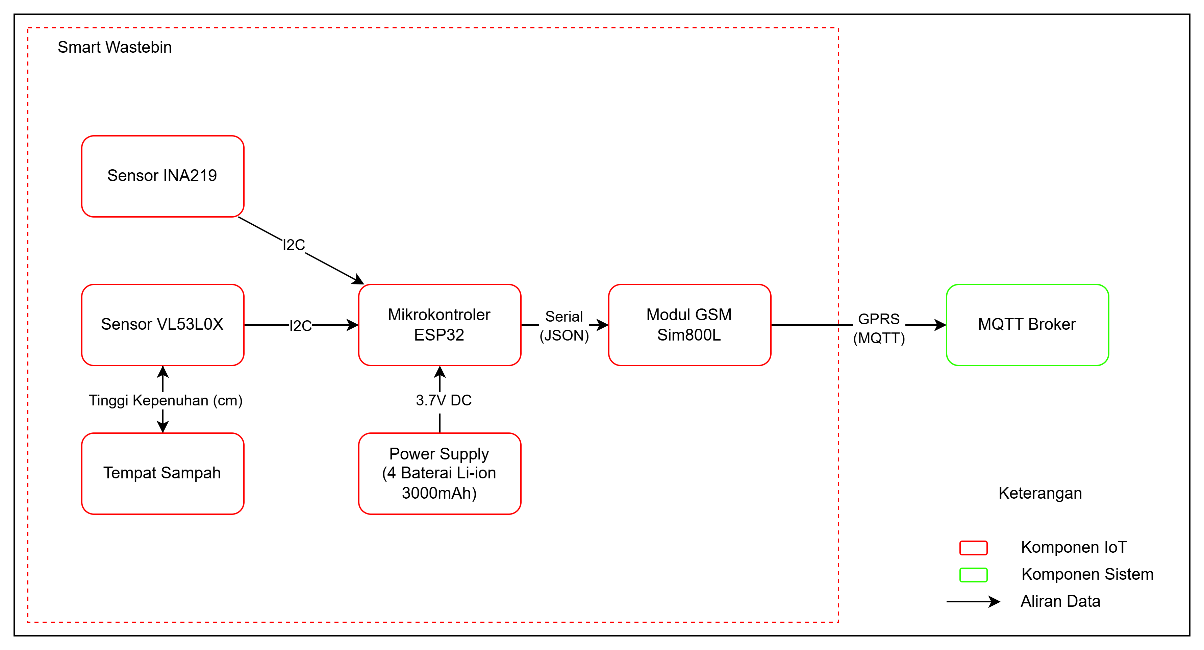
\includegraphics[width=0.85\textwidth]{images/blok-fungsional.png}
  % RENAME: image10.png → blok-fungsional.png
\end{figure}

Tabel \ref{tab:fungsi-komponen} menyajikan deskripsi fungsional setiap komponen perangkat.

\begin{table}[H]
  \caption{Fungsi Setiap Komponen \textit{Smart Waste Bin}}
  \label{tab:fungsi-komponen}
  \begin{tabularx}{\textwidth}{| l | X |}
    \hline
    \textbf{Komponen} & \textbf{Fungsi} \\
    \hline
    Sensor VL53L0X V2 & Mengukur jarak antara sensor dengan permukaan sampah \\
    \hline
    Sensor INA219 & Mengukur tegangan dan arus baterai untuk \textit{monitoring} daya \\
    \hline
    Mikrokontroler ESP32 & Memproses data sensor dan mengatur jadwal pengiriman \\
    \hline
    Modul GSM SIM800L & Mengirimkan data ke MQTT \textit{broker} melalui jaringan seluler \\
    \hline
    Baterai 18650 Li-Ion & Menyediakan sumber daya untuk seluruh komponen \\
    \hline
  \end{tabularx}
\end{table}

Mekanisme kerja perangkat secara fungsional adalah sebagai berikut. Setiap interval waktu tertentu, mikrokontroler terbangun dari mode \textit{deep sleep} dan mengaktifkan seluruh komponen. Sensor VL53L0X V2 melakukan pembacaan jarak, kemudian mikrokontroler mengambil nilai median untuk mengurangi \textit{noise}. Nilai jarak dikonversi menjadi persentase tingkat kepenuhan menggunakan Persamaan \ref{eq:fill-level}.

\begin{equation}
  \text{Fill Level} (\%) = \frac{\text{Kedalaman Bin} - \text{Jarak Terukur}}{\text{Kedalaman Bin}} \times 100
  \label{eq:fill-level}
\end{equation}
\eqcaption{Persamaan Konversi Tingkat Kepenuhan}

dengan kedalaman \textit{bin} sebesar 1000 mm. Persamaan ini memetakan seluruh rentang jarak terukur (0--1000 mm) menjadi nilai \textit{fillLevel} (0--100\%) secara linier dan kontinu, sehingga tidak terdapat rentang jarak yang tidak terdefinisi. Sebagai ilustrasi, Tabel \ref{tab:konversi-filllevel} menyajikan pemetaan beberapa rentang jarak terukur terhadap nilai \textit{fillLevel} yang dihasilkan.

\begin{table}[H]
  \caption{Pemetaan Jarak Terukur terhadap \textit{Fill Level}}
  \label{tab:konversi-filllevel}
  \centering
  \begin{tabular}{| c | c | c |}
    \hline
    \textbf{Jarak Terukur (mm)} & \textbf{\textit{Fill Level} (\%)} & \textbf{Interpretasi} \\
    \hline
    0--99 & 91--100 & Hampir penuh \\
    \hline
    100--299 & 71--90 & Terisi banyak \\
    \hline
    300--499 & 51--70 & Terisi sedang \\
    \hline
    500--699 & 31--50 & Terisi sebagian \\
    \hline
    700--899 & 11--30 & Hampir kosong \\
    \hline
    900--1000 & 0--10 & Kosong \\
    \hline
  \end{tabular}
\end{table}

Untuk menjaga validitas data, pembacaan jarak yang berada di luar rentang fisik \textit{bin} ditangani secara khusus. Jarak terukur yang melebihi 1000 mm (yang secara teoretis menghasilkan \textit{fillLevel} negatif) dibatasi (\textit{clamp}) menjadi 0\%, sedangkan pembacaan yang lebih kecil dari 0 mm dibatasi menjadi 100\%. Apabila sensor mengalami \textit{timeout} atau gagal melakukan pembacaan, nilai \textit{fillLevel} diisi dengan -1 sebagai penanda \textit{error}, yang kemudian disaring pada tahap praproses data. Dengan demikian, setiap kemungkinan nilai pembacaan, baik di dalam maupun di luar rentang valid, memiliki penanganan yang terdefinisi.

Sensor INA219 mengukur tegangan dan arus baterai untuk menghitung \textit{State of Charge} (SoC) menggunakan Persamaan \ref{eq:battery-percent}.

\begin{equation}
  \text{Battery Percent} (\%) = \frac{\text{Tegangan Terukur} - 5{,}60}{0{,}028}
  \label{eq:battery-percent}
\end{equation}
\eqcaption{Persamaan Perhitungan State of Charge Baterai}

Jika tegangan baterai di bawah 5,6V atau persentase di bawah 30\%, perangkat memasuki mode \textit{sleep forever} untuk mencegah kerusakan baterai akibat \textit{over-discharge}. Data yang telah diproses dikirimkan ke MQTT \textit{broker}, kemudian mikrokontroler kembali ke mode \textit{deep sleep}.

\subsection{Spesifikasi \textit{Interface} Data}

\textit{Interface} antara perangkat IoT dengan sistem internal didefinisikan melalui format data yang dikirimkan via protokol MQTT. Tabel \ref{tab:spesifikasi-mqtt} menyajikan spesifikasi koneksi MQTT yang digunakan.

\begin{table}[H]
  \caption{Spesifikasi Konektivitas MQTT}
  \label{tab:spesifikasi-mqtt}
  \begin{tabularx}{\textwidth}{| l | X |}
    \hline
    \textbf{Aspek} & \textbf{Nilai} \\
    \hline
    \textit{Broker} & Disediakan oleh vendor \\
    \hline
    \textit{Topic Pattern} & \texttt{wp2/basic\_01}; \texttt{wp2/basic\_02}; \texttt{wp2/basic\_03} \\
    \hline
    QoS \textit{Level} & 0 (default) \\
    \hline
    \textit{Authentication} & \textit{Username} dan \textit{password} (disediakan vendor) \\
    \hline
  \end{tabularx}
\end{table}

Data dikirimkan dalam format JSON. Tabel \ref{tab:payload-data} menyajikan spesifikasi setiap \textit{field} pada \textit{payload} data perangkat.

\begin{longtable}{| l | l | p{5.5cm} | l |}
  \caption{\textit{Payload} Data Perangkat}
  \label{tab:payload-data} \\
    \hline
    \textbf{\textit{Field}} & \textbf{Tipe Data} & \textbf{Deskripsi} & \textbf{Contoh} \\
    \hline
  \endfirsthead
    \hline
    \textbf{\textit{Field}} & \textbf{Tipe Data} & \textbf{Deskripsi} & \textbf{Contoh} \\
    \hline
  \endhead
    \hline
  \endfoot
    \texttt{sensor\_id} & String & Identifier unik perangkat & \texttt{"1"} \\
    \hline
    \texttt{tegangan} & Float & Tegangan baterai (Volt) & \texttt{7.25} \\
    \hline
    \texttt{arus} & Float & Arus perangkat (mA) & \texttt{100} \\
    \hline
    \texttt{daya} & Float & Daya terpakai (mW) & \texttt{727.4} \\
    \hline
    \texttt{battPercent} & Float & Persentase baterai (0--100) & \texttt{58.3} \\
    \hline
    \texttt{Ina219\_avail} & Boolean & Status ketersediaan sensor INA219 & \texttt{true} \\
    \hline
    \texttt{fillLevel} & Integer & Tingkat kepenuhan (0--100, atau -1 jika \textit{error}) & \texttt{65} \\
    \hline
    \texttt{dist} & Integer & Jarak terukur (mm, atau -1 jika \textit{error}) & \texttt{490} \\
    \hline
    \texttt{vol} & Integer & Volume sampah (dm³) & \texttt{38} \\
    \hline
    \texttt{sensor\_status} & String & Status sensor jarak & \texttt{"online"} \\
    \hline
    \texttt{vl53l0x\_avail} & Integer & Ketersediaan sensor (1=\textit{available}, 0=\textit{not}) & \texttt{1} \\
    \hline
    \texttt{event} & String & Tipe \textit{event} & \texttt{"DataUpdate"} \\
    \hline
\end{longtable}

Gambar \ref{fig:payload-contoh} menunjukkan contoh \textit{payload} data yang dikirimkan oleh perangkat.

\begin{figure}[H]
  \caption{Contoh \textit{Payload} Data Perangkat}
  \label{fig:payload-contoh}
  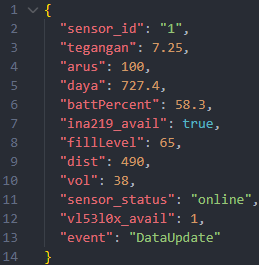
\includegraphics[width=0.45\textwidth]{images/payload-contoh.png}
  % RENAME: image11.png → payload-contoh.png
\end{figure}

% ============================================================
\section{Perancangan Adaptasi \textit{Firmware}}
\label{sec:perancangan-firmware}
% ============================================================

Sebagaimana diidentifikasi pada Subbab \ref{sec:analisis-kondisi}, perangkat \textit{Smart Waste Bin} yang tersedia memiliki konfigurasi \textit{firmware} yang dirancang untuk skala perkotaan. Untuk menyesuaikan dengan kebutuhan lingkungan kampus, dirancang lima adaptasi \textit{firmware}. Tabel \ref{tab:peningkatan-firmware} menyajikan ringkasan adaptasi yang dirancang.

\begin{table}[H]
  \caption{Rancangan Adaptasi \textit{Firmware}}
  \label{tab:peningkatan-firmware}
  \begin{tabularx}{\textwidth}{| X | X | X |}
    \hline
    \textbf{Aspek} & \textbf{Sebelum} & \textbf{Sesudah} \\
    \hline
    Interval Pengambilan Data & 8 jam & 2 jam 30 menit \\
    \hline
    Pembacaan Sensor & \textit{Single reading} & 5 \textit{readings} dengan \textit{median filter} \\
    \hline
    \textit{Error Handling} & Tidak ada mekanisme \textit{recovery} & \textit{Auto-recovery} dengan \textit{power cycle} \\
    \hline
    \textit{Warm-up} Sensor & Langsung pembacaan & 3x \textit{warm-up readings} sebelum pengukuran \\
    \hline
    Optimasi Daya & Standard GPIO & GPIO \textit{isolation} untuk mencegah \textit{floating} \\
    \hline
  \end{tabularx}
\end{table}

\subsection{Perancangan Perubahan Interval Pengambilan Data}

Interval pengambilan data pada kondisi awal adalah 8 jam, yang merupakan konfigurasi bawaan pada \textit{firmware} vendor (didefinisikan melalui konstanta \texttt{TIME\_TO\_SLEEP} pada kode sumber perangkat). Konfigurasi ini dirancang untuk konteks pemantauan kontainer sampah skala perkotaan yang volumenya besar dan laju pengisiannya lambat, sehingga pelaporan tiga kali sehari dinilai memadai oleh vendor sekaligus menghemat daya baterai.

Untuk konteks kampus, interval tersebut diubah menjadi 2 jam 30 menit berdasarkan pertimbangan berikut. Pertama, dari sisi kebutuhan resolusi data: dinamika pembuangan sampah kampus terkonsentrasi pada jam-jam tertentu dalam rentang jam aktif (sekitar 07:00--19:00), sehingga interval 8 jam yang hanya menghasilkan sekitar 3 titik data per hari berisiko melewatkan transisi antar sesi aktivitas (pagi, siang, sore). Interval 2,5 jam menghasilkan 8 sampai 9 titik data per hari, yang berarti terdapat sekitar 4--5 titik data dalam rentang jam aktif kampus, cukup untuk membedakan aktivitas antar sesi tanpa celah pengamatan yang lebar.

Kedua, dari sisi batasan daya: setiap siklus pengiriman mengaktifkan modul GSM SIM800L yang merupakan konsumen daya terbesar pada perangkat. Memperpendek interval lebih jauh (misalnya 1 jam, yang berarti 24 siklus per hari) akan melipatgandakan frekuensi aktivasi GSM hingga hampir tiga kali lipat dibandingkan interval 2,5 jam, sehingga secara proporsional memperpendek umur baterai dan meningkatkan frekuensi penggantian baterai di lapangan. Interval 2,5 jam dipilih sebagai titik keseimbangan: resolusi data memadai untuk analisis pola harian, sementara frekuensi aktivasi GSM (9--10 siklus per hari) masih berada pada tingkat yang memungkinkan perangkat beroperasi beberapa hari tanpa penggantian baterai. Dengan demikian, nilai 2,5 jam bukan angka arbitrer, melainkan hasil pertimbangan rekayasa antara kebutuhan resolusi analisis dan keterbatasan daya perangkat.

\subsection{Perancangan \textit{Median Filter}}

Pembacaan sensor VL53L0X ditingkatkan dari \textit{single reading} menjadi 5 kali pembacaan dengan pengambilan nilai median. Pendekatan ini dipilih karena median lebih \textit{robust} terhadap \textit{outlier} dibandingkan rata-rata (\textit{mean}). Mekanisme yang dirancang adalah sebagai berikut: sensor melakukan 5 kali pembacaan dengan interval 100ms, setiap pembacaan dicek validitasnya (\textit{timeout} dan \textit{range} 0--1400mm), nilai-nilai valid diurutkan, nilai median diambil sebagai hasil akhir, dan jika \textit{valid count} $<$ 3 digunakan rata-rata sebagai \textit{fallback}.

\subsection{Perancangan Mekanisme \textit{Auto-recovery}}

Sensor VL53L0X dapat mengalami kondisi \textit{hang} yang menyebabkan \textit{timeout} berulang. Kondisi \textit{trigger recovery} didefinisikan sebagai \textit{timeout} yang terjadi $\geq$ 3 kali dari 5 pembacaan, atau tidak ada pembacaan valid sama sekali. Langkah \textit{recovery} yang dirancang adalah: (1) \textit{stop continuous mode} pada sensor, (2) \textit{soft reset} dengan re-inisialisasi sensor, (3) jika \textit{soft reset} gagal, lakukan \textit{power cycle} (matikan daya sensor 500ms lalu hidupkan kembali), (4) re-inisialisasi I2C dan sensor, dan (5) jika masih gagal, tandai sensor sebagai \textit{offline}.

\subsection{Perancangan \textit{Warm-up} Sensor}

Sensor VL53L0X memerlukan beberapa pembacaan awal sebelum menghasilkan nilai yang stabil, karena pembacaan pertama setelah inisialisasi cenderung tidak representatif. Mekanisme \textit{warm-up} yang dirancang adalah: sensor diinisialisasi dan dikonfigurasi dengan \textit{timing budget} 200ms, mode \textit{continuous measurement} diaktifkan dengan interval 200ms, kemudian tiga pembacaan \textit{dummy} dilakukan dengan jeda 200ms per pembacaan tanpa menggunakan nilainya. Setelah \textit{warm-up} selesai, sensor dinyatakan siap untuk pengukuran aktual.

\subsection{Perancangan Optimasi Daya}

Dua mekanisme optimasi daya dirancang untuk memperpanjang masa operasi baterai. Pertama, \textit{GPIO Isolation}: sebelum \textit{deep sleep}, seluruh GPIO yang digunakan di-\textit{hold} pada kondisi LOW untuk mencegah \textit{floating state} yang dapat menyebabkan konsumsi daya tidak perlu. Kedua, \textit{proper shutdown sequence}: urutan mematikan komponen dioptimalkan untuk memastikan tidak ada komponen yang tertinggal dalam kondisi aktif. Tabel \ref{tab:urutan-shutdown} menyajikan urutan \textit{shutdown} yang dirancang.

\begin{table}[H]
  \caption{Urutan \textit{Shutdown} Perangkat}
  \label{tab:urutan-shutdown}
  \begin{tabularx}{\textwidth}{| l | l | X |}
    \hline
    \textbf{Step} & \textbf{Aksi} & \textbf{Keterangan} \\
    \hline
    1 & \textit{Stop} sensor \textit{continuous} & Menghentikan mode pembacaan kontinyu VL53L0X \\
    \hline
    2 & \textit{Disconnect} MQTT & Menutup koneksi MQTT dengan \textit{broker} \\
    \hline
    3 & GPRS \textit{disconnect} & Memutus koneksi data seluler \\
    \hline
    4 & Modem \textit{power off} & Mematikan modem SIM800L \\
    \hline
    5 & GPIO LOW & Set semua GPIO ke LOW (TRIG, TRIG\_SENSOR, LED) \\
    \hline
    6 & GPIO \textit{hold enable} & Isolasi GPIO untuk mencegah \textit{floating} saat \textit{sleep} \\
    \hline
    7 & I2C \textit{end} & Menonaktifkan bus I2C \\
    \hline
    8 & Serial \textit{flush} \& \textit{end} & \textit{Flush buffer} serial dan nonaktifkan \\
    \hline
    9 & \textit{Deep sleep} & Masuk mode \textit{deep sleep} selama 2,5 jam \\
    \hline
  \end{tabularx}
\end{table}

% ============================================================
\section{Perancangan \textit{Middleware}}
\label{sec:perancangan-middleware}
% ============================================================

\textit{Middleware} merupakan komponen internal yang berfungsi sebagai jembatan antara perangkat IoT pada \textit{Network Layer} dengan komponen penyimpanan pada \textit{Application Layer}. Pada sistem ini, \textit{middleware} dirancang menggunakan Node-RED. Subbab ini berfokus pada \emph{rancangan} arsitektur \textit{flow} serta \emph{spesifikasi target} konfigurasi \textit{node} yang menjadi acuan, sedangkan realisasi konfigurasi aktual beserta pengujiannya dibahas pada Bab \ref{chap:implementasi}.

\subsection{Arsitektur \textit{Flow} Node-RED}

\textit{Flow} Node-RED untuk sistem pemantauan sampah berbasis \textit{Internet of Things} dirancang untuk menerima data dari tiga perangkat sensor secara paralel dan meneruskannya ke \textit{database}. Gambar \ref{fig:flow-nodered} menunjukkan rancangan alur pemrosesan data secara konseptual, mulai dari penerimaan pesan hingga penyimpanan ke \textit{database}.

\begin{figure}[H]
  \caption{Rancangan Alur Pemrosesan Data \textit{Middleware}}
  \label{fig:flow-nodered}
  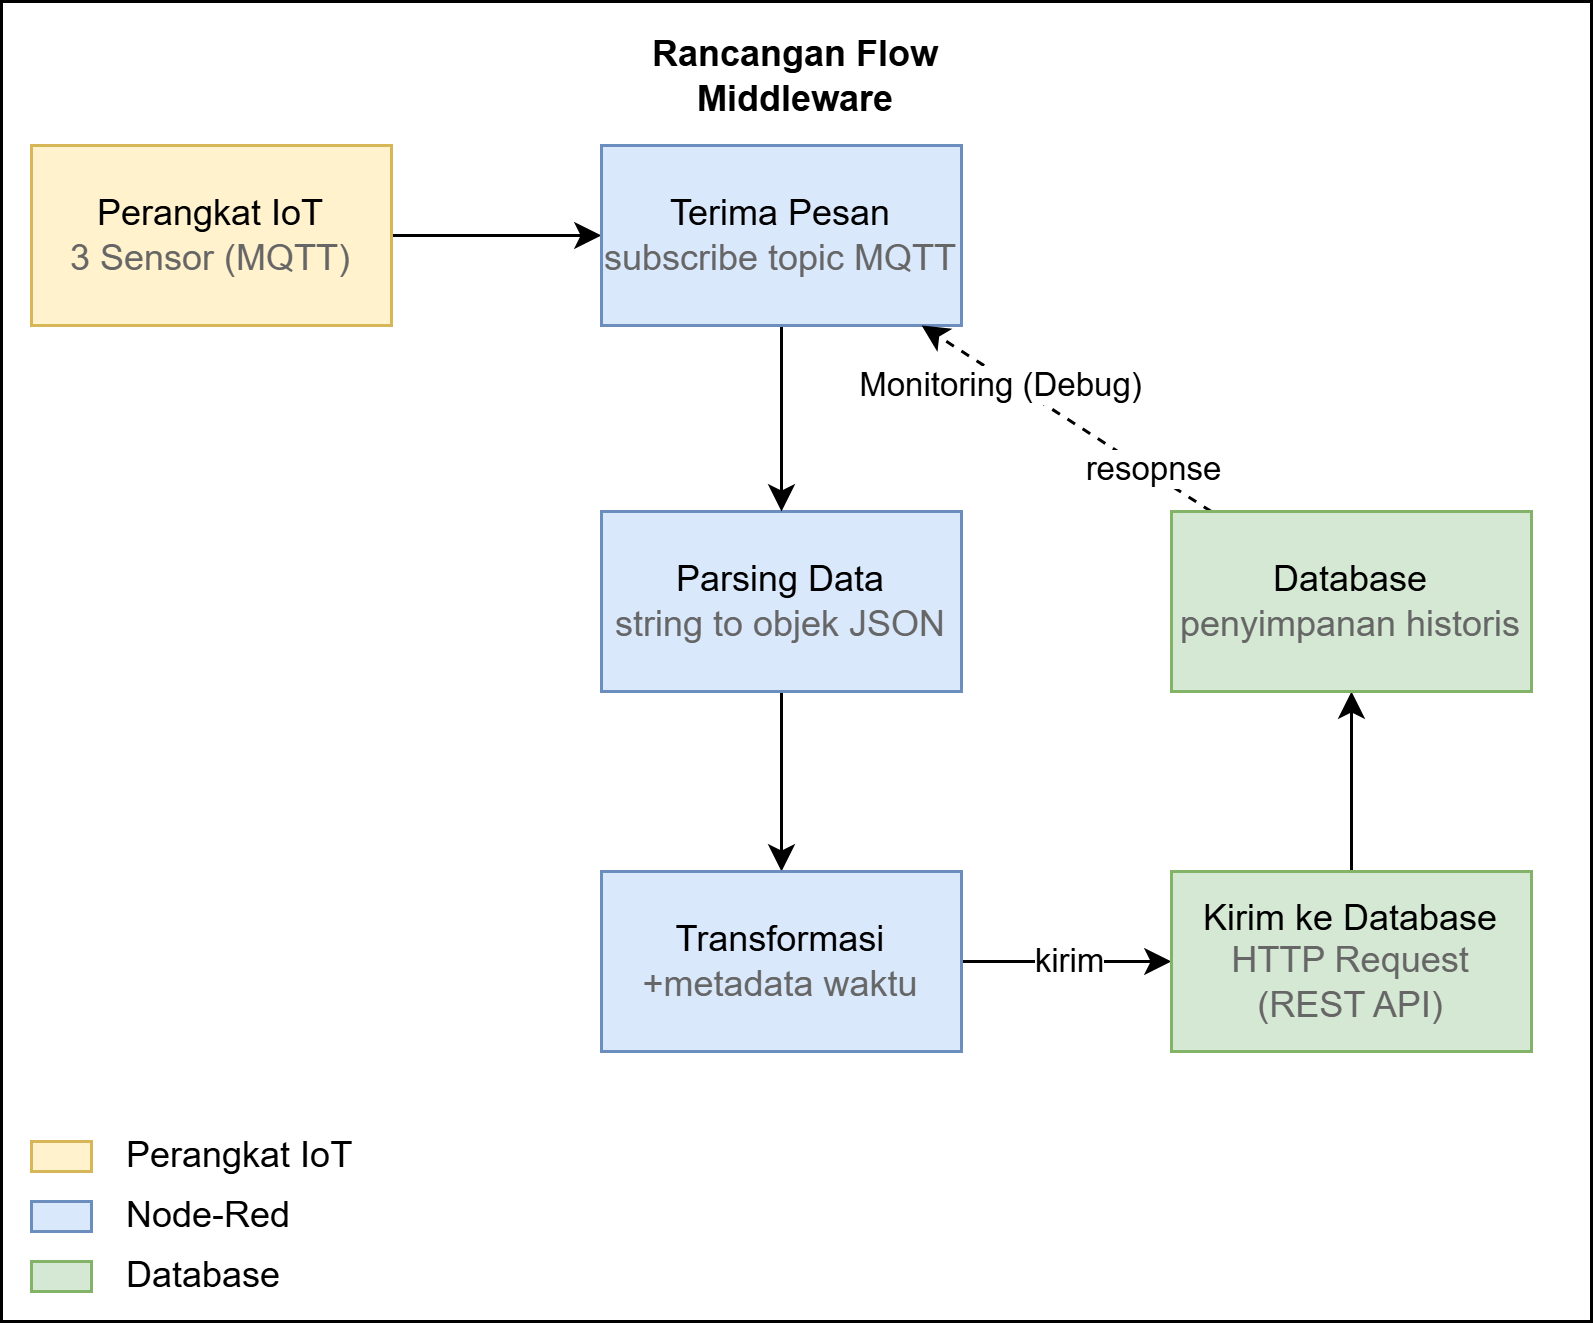
\includegraphics[width=\textwidth]{images/rancangan-flow-middleware.png}
  % CATATAN: gunakan diagram alur generik (mis. dibuat di draw.io),
  %          BUKAN tangkapan layar flow Node-RED yang sudah jadi.
  %          Tangkapan layar implementasi aktual ditempatkan di Bab V.
\end{figure}

Berdasarkan Gambar \ref{fig:flow-nodered}, \textit{middleware} dirancang menggunakan beberapa kelompok \textit{node} dengan peran yang berbeda. Tabel \ref{tab:tipe-node} menyajikan ringkasan tipe \textit{node} yang direncanakan beserta fungsinya.

\begin{table}[H]
  \caption{Tipe \textit{Node} pada \textit{Flow} Node-RED}
  \label{tab:tipe-node}
  \begin{tabularx}{\textwidth}{| l | l | X |}
    \hline
    \textbf{Tipe \textit{Node}} & \textbf{Jumlah} & \textbf{Fungsi} \\
    \hline
    Inject & 7 & Simulasi data untuk pengujian \\
    \hline
    MQTT In & 3 & Menerima data dari MQTT \textit{broker} \\
    \hline
    JSON & 3 & \textit{Parsing} string JSON ke objek \\
    \hline
    Function & 3 & Transformasi dan penambahan metadata \\
    \hline
    HTTP Request & 3 & Pengiriman data ke \textit{database} \\
    \hline
    Debug & 6 & \textit{Monitoring} data dan \textit{response} \\
    \hline
  \end{tabularx}
\end{table}

\subsection{Rancangan Alur Pemrosesan Data}

Alur pemrosesan data pada \textit{middleware} dirancang sebagai berikut. Pertama, pesan dari \textit{broker} MQTT diterima oleh \textit{node} penerima. Kedua, \textit{payload} dalam format string dikonversi menjadi objek terstruktur. Ketiga, dilakukan transformasi \textit{field} dan penambahan metadata berupa \textit{timestamp} server. Keempat, data yang telah diolah dikirimkan ke \textit{database} melalui REST API. \textit{Response} dari \textit{database} dipantau untuk memastikan keberhasilan penyimpanan. Spesifikasi konfigurasi aktual setiap \textit{node} beserta nilai parameternya dibahas pada Subbab \ref{sec:impl-middleware}.

\subsection{Spesifikasi \textit{Deployment} \textit{Middleware}}

Tabel \ref{tab:deployment-nodered} menyajikan spesifikasi \textit{deployment} dan operasional \textit{middleware} Node-RED yang direncanakan untuk sistem.

\begin{table}[H]
  \caption{Spesifikasi \textit{Deployment} dan Operasional Node-RED}
  \label{tab:deployment-nodered}
  \begin{tabularx}{\textwidth}{| l | X |}
    \hline
    \textbf{Aspek} & \textbf{Spesifikasi} \\
    \hline
    \textit{Platform} & Node-RED v4.1.3 \\
    \hline
    \textit{Runtime} & Node.js v24.12.0 \\
    \hline
    \textit{Hosting} & \textit{Server} lokal menggunakan komputer peneliti yang dinyalakan selama penelitian \\
    \hline
    \textit{Auto-connect} & \textit{Enabled} (reconnect otomatis ke MQTT \textit{broker}) \\
    \hline
    \textit{Flow} Name & MQTT to Supabase \textit{Flow} \\
    \hline
  \end{tabularx}
\end{table}

% ============================================================
\section{Perancangan \textit{Database}}
\label{sec:perancangan-database}
% ============================================================

\textit{Database} merupakan komponen pada \textit{Application Layer} yang berfungsi untuk menyimpan seluruh data pembacaan sensor secara persisten dan terstruktur. Sistem ini menggunakan Supabase yang merupakan \textit{platform Backend-as-a-Service} berbasis PostgreSQL.

\subsection{Spesifikasi \textit{Platform Database}}

Supabase dipilih karena menyediakan beberapa keunggulan: berbasis PostgreSQL sebagai \textit{database} relasional \textit{open source} dengan fitur lengkap, REST API \textit{built-in} yang memungkinkan akses data tanpa perlu mengembangkan \textit{backend} terpisah, dan \textit{dashboard} web untuk manajemen \textit{database}. Tabel \ref{tab:spesifikasi-database} menyajikan spesifikasi \textit{platform database}.

\begin{table}[H]
  \caption{Spesifikasi \textit{Platform Database}}
  \label{tab:spesifikasi-database}
  \begin{tabularx}{\textwidth}{| p{4cm} | X |}
    \hline
    \textbf{Aspek} & \textbf{Spesifikasi} \\
    \hline
    \textit{Platform} & Supabase \\
    \hline
    \textit{Database Engine} & PostgreSQL \\
    \hline
    \textit{Hosting} & Supabase \textit{Cloud} (Free Tier) \\
    \hline
    Akses Data & REST API (PostgREST) \\
    \hline
    Autentikasi API & API Key (anon key) \\
    \hline
    \textit{Dashboard} & \textit{Web-based} \\
    \hline
  \end{tabularx}
\end{table}

\subsection{Desain Skema \textit{Database}}

Sistem menggunakan satu tabel utama bernama \texttt{sensor\_data} untuk menyimpan seluruh data pembacaan sensor. Desain ini dipilih karena data yang dikumpulkan bersifat \textit{time-series} dengan struktur yang seragam dari semua perangkat. Gambar \ref{fig:tabel-sensordata} menunjukkan struktur tabel \texttt{sensor\_data}.

\begin{figure}[H]
  \caption{Struktur Tabel \texttt{sensor\_data} pada Supabase}
  \label{fig:tabel-sensordata}
  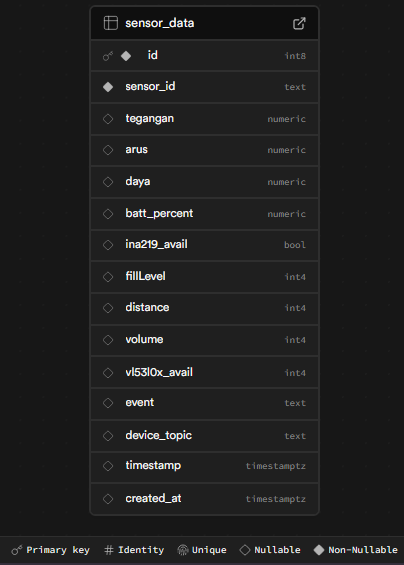
\includegraphics[width=0.5\textwidth]{images/tabel-sensordata.png}
  % RENAME: image13.png → tabel-sensordata.png
\end{figure}

Tabel \ref{tab:detail-sensordata} menyajikan spesifikasi setiap kolom pada tabel \texttt{sensor\_data}.

\begin{longtable}{| p{2.6cm} | p{1.8cm} | p{2.6cm} | p{5cm} |}
  \caption{Detail Kolom Tabel \texttt{sensor\_data}}
  \label{tab:detail-sensordata} \\
    \hline
    \textbf{Kolom} & \textbf{Tipe Data} & \textbf{\textit{Constraint}} & \textbf{Deskripsi} \\
    \hline
  \endfirsthead
    \hline
    \textbf{Kolom} & \textbf{Tipe Data} & \textbf{\textit{Constraint}} & \textbf{Deskripsi} \\
    \hline
  \endhead
    \hline
  \endfoot
    \texttt{id} & int8 & PK, Auto-increment & Identifier unik record \\
    \hline
    \texttt{sensor\_id} & text & Not Null & Identifier perangkat sensor \\
    \hline
    \texttt{tegangan} & Numeric & Nullable & Tegangan baterai (Volt) \\
    \hline
    \texttt{arus} & Numeric & Nullable & Arus baterai (mA) \\
    \hline
    \texttt{daya} & Numeric & Nullable & Daya terpakai (mW) \\
    \hline
    \texttt{batt\_percent} & Numeric & Nullable & Persentase baterai (\%) \\
    \hline
    \texttt{ina219\_avail} & Bool & Nullable & Status ketersediaan sensor INA219 \\
    \hline
    \texttt{fillLevel} & Int4 & Nullable & Tingkat kepenuhan (0--100\%) \\
    \hline
    \texttt{distance} & Int4 & Nullable & Jarak terukur (mm) \\
    \hline
    \texttt{volume} & Int4 & Nullable & Volume sampah (dm³) \\
    \hline
    \texttt{vl53l0x\_avail} & Int4 & Nullable & Ketersediaan sensor VL53L0X (1/0) \\
    \hline
    \texttt{event} & text & Nullable & Tipe \textit{event} (DataUpdate, LowBattery, dll.) \\
    \hline
    \texttt{device\_topic} & text & Nullable & \textit{Topic} MQTT sumber data \\
    \hline
    \texttt{timestamp} & timestamptz & Nullable & Waktu pembacaan sensor (dari perangkat) \\
    \hline
    \texttt{created\_at} & timestamptz & Nullable & Waktu data disimpan di \textit{database} \\
    \hline
\end{longtable}

\textit{Field} \texttt{timestamp} mencatat waktu pembacaan di perangkat IoT, sedangkan \texttt{created\_at} mencatat waktu data diterima dan disimpan di \textit{database}. Selisih antara kedua \textit{timestamp} tersebut menunjukkan latensi transmisi data dari perangkat ke \textit{database}.

% ============================================================
\section{Perancangan \textit{Dashboard}}
\label{sec:perancangan-dashboard}
% ============================================================

\textit{Dashboard} merupakan komponen pada \textit{Application Layer} yang berfungsi sebagai antarmuka pengguna untuk memvisualisasikan data sensor. Sistem ini menggunakan Next.js sebagai \textit{framework} utama.

\subsection{Arsitektur \textit{Dashboard}}

\textit{Dashboard} dibangun menggunakan arsitektur \textit{client-server} dengan Next.js. Komponen \textit{frontend} mengambil data dari \textit{backend} melalui API Routes yang terhubung ke \textit{database} Supabase menggunakan Drizzle ORM. Tabel \ref{tab:teknologi-dashboard} menyajikan komponen teknologi yang digunakan.

\begin{table}[H]
  \caption{Komponen Teknologi \textit{Dashboard}}
  \label{tab:teknologi-dashboard}
  \begin{tabularx}{\textwidth}{| l | l | X |}
    \hline
    \textbf{Komponen} & \textbf{Teknologi} & \textbf{Fungsi} \\
    \hline
    Framework & Next.js & \textit{Server-side rendering} dan routing \\
    \hline
    UI \textit{Library} & React & Komponen antarmuka pengguna \\
    \hline
    Styling & Tailwind CSS & CSS framework \\
    \hline
    \textit{Charting} & Recharts & \textit{Library} visualisasi data \\
    \hline
    ORM & Drizzle ORM & \textit{Object-Relational Mapping} untuk akses \textit{database} \\
    \hline
    \textit{Database} & Supabase PostgreSQL & Penyimpanan data \\
    \hline
  \end{tabularx}
\end{table}

\subsection{Perancangan API}

\textit{Dashboard} berkomunikasi dengan \textit{database} melalui API Routes pada endpoint \texttt{/api/sensor-data}. Tabel \ref{tab:spesifikasi-api} menyajikan spesifikasi API \textit{endpoint} yang dirancang.

\begin{table}[H]
  \caption{Spesifikasi API \textit{Endpoint}}
  \label{tab:spesifikasi-api}
  \begin{tabularx}{\textwidth}{| l | l | X |}
    \hline
    \textbf{Metode} & \textbf{Parameter} & \textbf{Fungsi} \\
    \hline
    GET & \texttt{sensorId}, \texttt{timerange}, \texttt{limit} & Mengambil data sensor dengan \textit{filter} \\
    \hline
    POST & Body: sensor data object & Menyimpan data sensor baru \\
    \hline
    PUT & Body: id, update \textit{fields} & Memperbarui data sensor \\
    \hline
    DELETE & \texttt{id}, \texttt{sensorId}, \texttt{olderThan} & Menghapus data sensor \\
    \hline
  \end{tabularx}
\end{table}

API GET mendukung parameter \texttt{timerange} dengan nilai sebagaimana pada Tabel \ref{tab:parameter-timerange}.

\begin{table}[H]
  \caption{Nilai Parameter \texttt{timerange}}
  \label{tab:parameter-timerange}
  \begin{tabularx}{\textwidth}{| l | X |}
    \hline
    \textbf{Nilai} & \textbf{Rentang Waktu} \\
    \hline
    \texttt{1h} & 1 jam terakhir \\
    \hline
    \texttt{24h} & 24 jam terakhir (\textit{default}) \\
    \hline
    \texttt{7d} & 7 hari terakhir \\
    \hline
    \texttt{30d} & 30 hari terakhir \\
    \hline
  \end{tabularx}
\end{table}

\subsection{Perancangan Antarmuka}

Antarmuka \textit{dashboard} dirancang terdiri dari enam komponen utama:

\begin{enumerate}
  \item \textbf{\textit{Header Section}}: menampilkan judul aplikasi, tombol \textit{refresh} manual, dan informasi \textit{timestamp} pembaruan terakhir.
  \item \textbf{\textit{Sensor Status Cards}}: kartu status untuk setiap sensor aktif, menampilkan \textit{fill level} dengan \textit{progress bar} berwarna (hijau $\leq$70\%, kuning 71--85\%, merah $>$85\%), persentase baterai, konsumsi daya, \textit{topic} MQTT, dan \textit{timestamp} terakhir.
  \item \textbf{\textit{Control Panel}}: \textit{dropdown} pemilihan sensor dan rentang waktu, serta informasi jumlah \textit{data points} dan \textit{active sensors}.
  \item \textbf{Visualisasi Data}: dua \textit{chart} interaktif, yaitu \textit{line chart} tren tingkat kepenuhan dan \textit{dual-axis line chart} baterai dan konsumsi daya.
  \item \textbf{\textit{Recent Sensor Readings}}: tabel 10 pembacaan terbaru dengan \textit{progress bar} mini dan \textit{status indicator}.
  \item \textbf{\textit{System Analytics}}: lima metrik agregat sistem (Total Records, Active Sensors, Avg Battery, Avg Power, Critical Alerts).
\end{enumerate}

\textit{Dashboard} dirancang dengan \textit{auto-refresh} setiap 30 detik menggunakan \texttt{useEffect} Hook dengan \textit{cleanup function} untuk mencegah \textit{memory leak}.

\subsection{Spesifikasi \textit{Hosting Dashboard}}

Tabel \ref{tab:hosting-dashboard} menyajikan spesifikasi \textit{hosting} \textit{dashboard} pada \textit{platform} Vercel.

\begin{table}[H]
  \caption{Spesifikasi \textit{Hosting Dashboard}}
  \label{tab:hosting-dashboard}
  \begin{tabularx}{\textwidth}{| l | X |}
    \hline
    \textbf{Aspek} & \textbf{Spesifikasi} \\
    \hline
    \textit{Platform} & Vercel (\textit{free tier}) \\
    \hline
    \textit{Framework Preset} & Next.js \\
    \hline
    \textit{Build Command} & \texttt{next build} \\
    \hline
    \textit{Output Directory} & \texttt{.next} \\
    \hline
    \textit{Deployment Method} & Git Integration (\textit{Continuous Deployment}) \\
    \hline
    Domain & Subdomain Vercel (\texttt{*.vercel.app}) \\
    \hline
  \end{tabularx}
\end{table}

\textit{Deployment} dilakukan secara otomatis melalui integrasi dengan repositori Git. Setiap \textit{push} ke \textit{branch} utama akan memicu proses \textit{build} dan \textit{deployment} secara otomatis (\textit{Continuous Deployment}).